% !TEX encoding = UTF-8
% !TEX TS-program = pdflatex
% !TEX root = ../tesi.tex

%**************************************************************
\chapter{L'azienda}
\label{cap:processi-metodologie}

\section{Profilo}
Web PD s.a.s. é una software house nata nel 2009, con sede a Padova ma con clienti in tutta Italia. La società nasce con lo scopo di gestire portali ecommerce, ma negli anni ha modificato la sua key activity in sviluppo di soluzioni software personalizzate. Ad oggi si occupa di consulenza informatica su software gestionali, applicazioni web e mobile (sia Android che iOS).\\
\begin{figure}[!h] 
	\centering 
	
\includegraphics[width=0.4\columnwidth]{azienda/logo_webpd} 
	\caption{Logo WebPD}
\end{figure}
\\
Il primo prodotto realizzato da Web PD é il gestionale Martina, un software per piattaforma Windows, sviluppato secondo un’architettura client-server modulare, che consente la gestione del ciclo attivo (vendite) e passivo (acquisti) di un’impresa commerciale. Grazie alla sua struttura modulare, é possibile aggiungere a Martina diverse funzionalità, come ad esempio gestione di magazzino, gestione della contabilità e
gestione dello scadenziario.\\
\\
Successivamente l’azienda aggiunge al portfolio di servizi offerti anche la realizzazione, grazie alle piattaforme OpenCart e Prestashop, di siti e-commerce integrati al gestionale Martina. \\
È in questo contesto che prima nascono gli ecommerce TuttoNauticaWeb.com e MiglioNautico.com, successivamente FarmaZero.com e SubitoStore.com.\\
\\
Nel 2015 Web PD da s.a.s. si trasforma in s.r.l. perché ha l’intenzione di addentrarsi nel settore turistico; questa strategia si perfeziona con l’acquisizione di un agenzia di viaggi ad Albignasego (PD).\\
\\
Nel 2016 il network e franchising di agenzie di viaggio Primarete Viaggi e Vacanze s.r.l. acquisisce il 49\% delle quote sociali di Web PD s.r.l.. Il frutto di questa collaborazione é l’ammodernamento, continuo ed ancora in corso, dei portali Viaggiregalo.it, CrociereRegalo.it, SimaWorldTravel.it e PercorsiReligiosi.it, di proprietà di Promoter Travel s.r.l., una controllata di Primarete.\\

\section{Dominio tecnologico}
L'azienda offre un ampio ventaglio di prodotti, che coinvolgono diverse piattaforme. È opportuno esaminare le tecnologie adoperate raggruppandole nelle seguenti categorie: \textit{Web}, \textit{Mobile} e \textit{Desktop}.

\subsection{Web}
In WebPD, la realizzazione di prodotti basati su piattaforma Web avviene, a livello di backend, utilizzando come linguaggio di programmazione PHP (versione 5 o 7). Molto spesso, per i progetti più complessi, viene usato il framework \textit{Codeigniter} (versione 3), che agevola l'implementazione del design pattern MVC e fornisce numerosi strumenti per facilitare (dunque accellerare) lo sviluppo. Codeigniter, tra le altre cose, infatti, implementa una serie di classi che facilitano l'esecuzione ed il debug delle query, oltre ad un meccanismo che permette di salvarle in cache (aumentando notevolmente le prestazioni del prodotto).\\
\begin{figure}[!h] 
	\centering 
	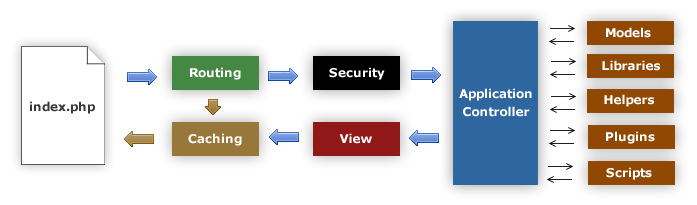
\includegraphics[width=1.0\columnwidth]{azienda/codeigniter_flow} 
	\caption{Flow chart di un'applicazione creata con Codeigniter}
\end{figure}\\
Per quanto riguarda il frontend, invece, viene utilizzato HTML5, CSS3 e Javascript (jQuery), senza usare framework che implementino Single Page Application (come React.js o Angular).\\\\\
Come server web, infine, vengono usati \textit{Apache2}, in caso di hosting su piattaforma Linux, o  \textit{IIS}, in caso di hosting su piattaforma Windows.\\\\
Per la realizzazione di siti web semplici, dove per semplici si intende senza esigenze di svolgimento di operazioni complesse, viene prediletto l'utilizzo di CMS, quali Wordpress (nel caso di blog, vetrine o forum) e OpenChart (nel caso di siti di e-commerce).
\\
\\
\subsubsection{DBMS}
Per lo sviluppo di prodotti software, WebPD si appoggia a due DBMS: \textit{Microsoft SQL Server 2012} e \textit{MySQL Server}. Entrambi questi software sono RDBMS, ma la scelta di utilizzare l'uno o l'altro dipende dalle caratteristiche del progetto, nello specifico: \begin{itemize}
	\item \textbf{Microsoft SQL Server} viene utilizzato nei progetti che prevedono un'ampia mole di dati da gestire e interrogazioni (query) complesse (come, ad esempio, CrociereRegalo.it), in quanto in tali contesti si è dimostrato mediamente più performante di \textit{MySQL};
	\item \textbf{MySQL Server} viene utilizzato il più possibile in caso il progetto non contenga una grossa mole di dati e/o interrogazioni complesse, in quanto non prevede costi di licenza (mentre \textit{SQL Server} si, e anche abbastanza elevati \footcite{site:sql-server-pricing}) ed é multipiattaforma (attualmente disponibile per Linux, Windows e MacOS).
\end{itemize}

\subsection{Mobile}
Il know-how accumulato da WebPD nella realizzazione di applicazioni web ha portato all'adozione del framework \textit{Cordova} per la creazione di applicazioni mobile, il quale offre la possibilità di creare app ibride cross platform utilizzando HTML/CSS e Javascript. Tali applicazioni, grazie ad alcune interfacce messe a disposizione da Cordova, possono accedere alle funzionalità native del dispositivo, come fotocamera, storage o sensoristica varia (accellerometro, giroscopio e GPS, se presenti).

\begin{figure}[!h] 
	\centering 
	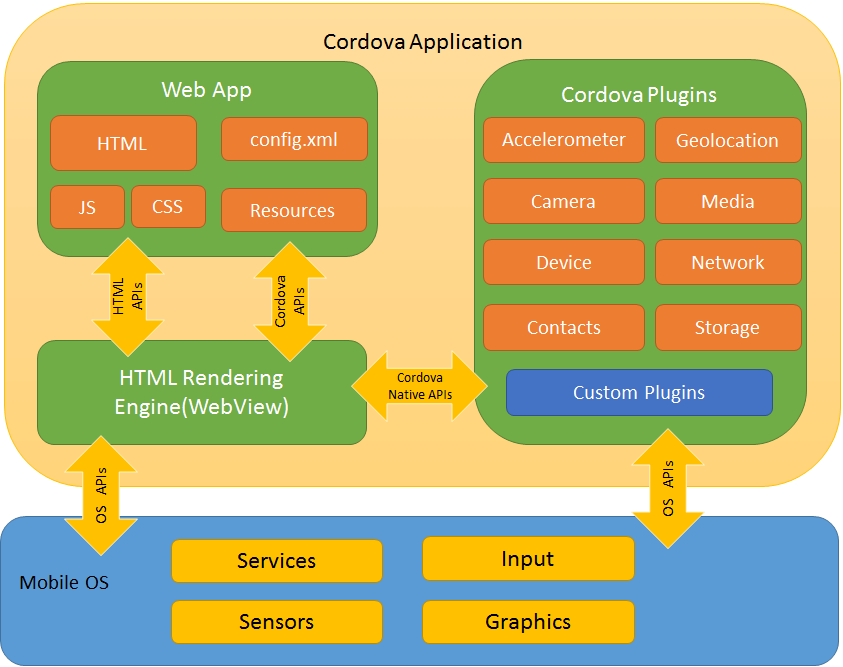
\includegraphics[width=0.6\columnwidth]{azienda/cordova_architettura} 
	\caption{Schema dell'architettura di un'app basata su Cordova}
\end{figure}

\subsection{Desktop}
La realizzazione di applicazioni desktop avviene attraverso l'utilizzo di due linguaggi: Java e Delphi.\\
Delphi viene usato soprattutto quando i programmi necessitano di manipolare grandi basi di dati, in quanto le applicazioni sono compilate in binario, quindi mediamente più performanti, e il linguaggio possiede numerose librerie che ne facilitano l'accesso.\\
Java, di contro, viene usato quando si ha l'esigenza di creare applicazioni cross-platform che non coinvolgano grandi volumi di dati.
\section{Processi di sviluppo}